% Options for packages loaded elsewhere
\PassOptionsToPackage{unicode}{hyperref}
\PassOptionsToPackage{hyphens}{url}
%
\documentclass[
]{article}
\usepackage{amsmath,amssymb}
\usepackage{iftex}
\ifPDFTeX
  \usepackage[T1]{fontenc}
  \usepackage[utf8]{inputenc}
  \usepackage{textcomp} % provide euro and other symbols
\else % if luatex or xetex
  \usepackage{unicode-math} % this also loads fontspec
  \defaultfontfeatures{Scale=MatchLowercase}
  \defaultfontfeatures[\rmfamily]{Ligatures=TeX,Scale=1}
\fi
\usepackage{lmodern}
\ifPDFTeX\else
  % xetex/luatex font selection
\fi
% Use upquote if available, for straight quotes in verbatim environments
\IfFileExists{upquote.sty}{\usepackage{upquote}}{}
\IfFileExists{microtype.sty}{% use microtype if available
  \usepackage[]{microtype}
  \UseMicrotypeSet[protrusion]{basicmath} % disable protrusion for tt fonts
}{}
\makeatletter
\@ifundefined{KOMAClassName}{% if non-KOMA class
  \IfFileExists{parskip.sty}{%
    \usepackage{parskip}
  }{% else
    \setlength{\parindent}{0pt}
    \setlength{\parskip}{6pt plus 2pt minus 1pt}}
}{% if KOMA class
  \KOMAoptions{parskip=half}}
\makeatother
\usepackage{xcolor}
\usepackage[margin=1in]{geometry}
\usepackage{color}
\usepackage{fancyvrb}
\newcommand{\VerbBar}{|}
\newcommand{\VERB}{\Verb[commandchars=\\\{\}]}
\DefineVerbatimEnvironment{Highlighting}{Verbatim}{commandchars=\\\{\}}
% Add ',fontsize=\small' for more characters per line
\usepackage{framed}
\definecolor{shadecolor}{RGB}{248,248,248}
\newenvironment{Shaded}{\begin{snugshade}}{\end{snugshade}}
\newcommand{\AlertTok}[1]{\textcolor[rgb]{0.94,0.16,0.16}{#1}}
\newcommand{\AnnotationTok}[1]{\textcolor[rgb]{0.56,0.35,0.01}{\textbf{\textit{#1}}}}
\newcommand{\AttributeTok}[1]{\textcolor[rgb]{0.13,0.29,0.53}{#1}}
\newcommand{\BaseNTok}[1]{\textcolor[rgb]{0.00,0.00,0.81}{#1}}
\newcommand{\BuiltInTok}[1]{#1}
\newcommand{\CharTok}[1]{\textcolor[rgb]{0.31,0.60,0.02}{#1}}
\newcommand{\CommentTok}[1]{\textcolor[rgb]{0.56,0.35,0.01}{\textit{#1}}}
\newcommand{\CommentVarTok}[1]{\textcolor[rgb]{0.56,0.35,0.01}{\textbf{\textit{#1}}}}
\newcommand{\ConstantTok}[1]{\textcolor[rgb]{0.56,0.35,0.01}{#1}}
\newcommand{\ControlFlowTok}[1]{\textcolor[rgb]{0.13,0.29,0.53}{\textbf{#1}}}
\newcommand{\DataTypeTok}[1]{\textcolor[rgb]{0.13,0.29,0.53}{#1}}
\newcommand{\DecValTok}[1]{\textcolor[rgb]{0.00,0.00,0.81}{#1}}
\newcommand{\DocumentationTok}[1]{\textcolor[rgb]{0.56,0.35,0.01}{\textbf{\textit{#1}}}}
\newcommand{\ErrorTok}[1]{\textcolor[rgb]{0.64,0.00,0.00}{\textbf{#1}}}
\newcommand{\ExtensionTok}[1]{#1}
\newcommand{\FloatTok}[1]{\textcolor[rgb]{0.00,0.00,0.81}{#1}}
\newcommand{\FunctionTok}[1]{\textcolor[rgb]{0.13,0.29,0.53}{\textbf{#1}}}
\newcommand{\ImportTok}[1]{#1}
\newcommand{\InformationTok}[1]{\textcolor[rgb]{0.56,0.35,0.01}{\textbf{\textit{#1}}}}
\newcommand{\KeywordTok}[1]{\textcolor[rgb]{0.13,0.29,0.53}{\textbf{#1}}}
\newcommand{\NormalTok}[1]{#1}
\newcommand{\OperatorTok}[1]{\textcolor[rgb]{0.81,0.36,0.00}{\textbf{#1}}}
\newcommand{\OtherTok}[1]{\textcolor[rgb]{0.56,0.35,0.01}{#1}}
\newcommand{\PreprocessorTok}[1]{\textcolor[rgb]{0.56,0.35,0.01}{\textit{#1}}}
\newcommand{\RegionMarkerTok}[1]{#1}
\newcommand{\SpecialCharTok}[1]{\textcolor[rgb]{0.81,0.36,0.00}{\textbf{#1}}}
\newcommand{\SpecialStringTok}[1]{\textcolor[rgb]{0.31,0.60,0.02}{#1}}
\newcommand{\StringTok}[1]{\textcolor[rgb]{0.31,0.60,0.02}{#1}}
\newcommand{\VariableTok}[1]{\textcolor[rgb]{0.00,0.00,0.00}{#1}}
\newcommand{\VerbatimStringTok}[1]{\textcolor[rgb]{0.31,0.60,0.02}{#1}}
\newcommand{\WarningTok}[1]{\textcolor[rgb]{0.56,0.35,0.01}{\textbf{\textit{#1}}}}
\usepackage{graphicx}
\makeatletter
\def\maxwidth{\ifdim\Gin@nat@width>\linewidth\linewidth\else\Gin@nat@width\fi}
\def\maxheight{\ifdim\Gin@nat@height>\textheight\textheight\else\Gin@nat@height\fi}
\makeatother
% Scale images if necessary, so that they will not overflow the page
% margins by default, and it is still possible to overwrite the defaults
% using explicit options in \includegraphics[width, height, ...]{}
\setkeys{Gin}{width=\maxwidth,height=\maxheight,keepaspectratio}
% Set default figure placement to htbp
\makeatletter
\def\fps@figure{htbp}
\makeatother
\setlength{\emergencystretch}{3em} % prevent overfull lines
\providecommand{\tightlist}{%
  \setlength{\itemsep}{0pt}\setlength{\parskip}{0pt}}
\setcounter{secnumdepth}{5}
\ifLuaTeX
  \usepackage{selnolig}  % disable illegal ligatures
\fi
\IfFileExists{bookmark.sty}{\usepackage{bookmark}}{\usepackage{hyperref}}
\IfFileExists{xurl.sty}{\usepackage{xurl}}{} % add URL line breaks if available
\urlstyle{same}
\hypersetup{
  pdftitle={Project : ConnectZA Churn Prediction},
  pdfauthor={Nduduzo Simangaliso Mthimkhulu},
  hidelinks,
  pdfcreator={LaTeX via pandoc}}

\title{Project : ConnectZA Churn Prediction}
\author{Nduduzo Simangaliso Mthimkhulu}
\date{}

\begin{document}
\maketitle

\newpage

\hypertarget{data-exploration-and-preparation}{%
\subsection{DATA EXPLORATION AND
PREPARATION}\label{data-exploration-and-preparation}}

\begin{Shaded}
\begin{Highlighting}[]
\FunctionTok{rm}\NormalTok{(}\AttributeTok{list =} \FunctionTok{ls}\NormalTok{())}

\CommentTok{\#Load data set}
\NormalTok{customer.data }\OtherTok{\textless{}{-}} \FunctionTok{read.csv}\NormalTok{(}\StringTok{"connectza\_churn\_data.csv"}\NormalTok{, }\AttributeTok{row.names =} \DecValTok{1}\NormalTok{)}

\CommentTok{\#Display structure}
\FunctionTok{str}\NormalTok{(customer.data)}
\end{Highlighting}
\end{Shaded}

\begin{verbatim}
## 'data.frame':    1000 obs. of  8 variables:
##  $ Age                    : int  54 31 42 46 43 37 56 37 62 37 ...
##  $ SubscriptionTier       : chr  "Premium" "Standard" "Basic" "Premium" ...
##  $ ContractDuration_Months: int  18 24 12 3 18 3 4 6 12 18 ...
##  $ DataUsage_GB           : num  52.6 13.3 0.3 5.4 5.2 5.8 0.7 12 2.1 18.8 ...
##  $ UsageFrequency         : num  19 8.6 6.5 22.4 3.8 4.5 6.5 6.3 4.6 10.4 ...
##  $ SupportTickets         : int  2 3 1 2 2 3 0 4 3 3 ...
##  $ SatisfactionScore      : int  7 7 8 6 8 7 7 6 6 7 ...
##  $ Churn                  : int  0 0 0 0 0 0 0 0 0 0 ...
\end{verbatim}

\hfill\break
\textbf{CustomerID}: This is just a unique identifier for each customer.
It's useful for tracking, but it won't help with prediction, so we won't
include it in modelling.

\textbf{Churn}: This is the main variable we're trying to predict. A
value of 1 means the customer left (churned), and 0 means they stayed.
It's a binary outcome.

\textbf{UsageFrequency}: This tells us how often a customer uses the
service each week, low frequency may indicate disengagement.

\textbf{SupportTickets}: This is the number of support queries raised in
the last 3 months.high tickets signal service issues.

\textbf{Age}: The age of the customer. This might influence how
comfortable they are with tech or how likely they are to explore other
providers.

\textbf{SubscriptionTier}: Package type (Basic, Standard, Premium);
higher tiers may reflect loyalty or higher value

\textbf{SatisfactionScore}: Customer survey rating (1-10); low scores
predict churn due to poor experience.

\textbf{DataUsage\_GB}: This is how much data the customer uses per
month. People who use more data might depend more on the service and be
less likely to switch providers.

\textbf{ContractDuration\_Months}: Contract length; longer contracts
suggest commitment, lowering churn risk.\\

\begin{Shaded}
\begin{Highlighting}[]
\CommentTok{\#summary statistics for all variables(WITH VISUALISATION )}
\FunctionTok{summary}\NormalTok{(customer.data)}
\end{Highlighting}
\end{Shaded}

\begin{verbatim}
##       Age        SubscriptionTier   ContractDuration_Months  DataUsage_GB  
##  Min.   :18.00   Length:1000        Min.   : 1.00           Min.   :  0.0  
##  1st Qu.:30.00   Class :character   1st Qu.: 6.00           1st Qu.:  2.1  
##  Median :38.00   Mode  :character   Median :12.00           Median :  5.4  
##  Mean   :37.97                      Mean   :15.25           Mean   : 10.4  
##  3rd Qu.:46.00                      3rd Qu.:18.00           3rd Qu.: 12.1  
##  Max.   :80.00                      Max.   :36.00           Max.   :185.8  
##  UsageFrequency   SupportTickets   SatisfactionScore     Churn      
##  Min.   : 1.000   Min.   : 0.000   Min.   : 2.000    Min.   :0.000  
##  1st Qu.: 5.375   1st Qu.: 1.000   1st Qu.: 5.000    1st Qu.:0.000  
##  Median : 8.000   Median : 2.000   Median : 6.000    Median :0.000  
##  Mean   : 8.933   Mean   : 2.245   Mean   : 6.212    Mean   :0.134  
##  3rd Qu.:11.425   3rd Qu.: 3.000   3rd Qu.: 7.000    3rd Qu.:0.000  
##  Max.   :28.000   Max.   :10.000   Max.   :10.000    Max.   :1.000
\end{verbatim}

\begin{Shaded}
\begin{Highlighting}[]
\NormalTok{churn\_rate }\OtherTok{\textless{}{-}} \FunctionTok{mean}\NormalTok{(customer.data}\SpecialCharTok{$}\NormalTok{Churn) }\SpecialCharTok{*} \DecValTok{100}
\NormalTok{churn\_rate}
\end{Highlighting}
\end{Shaded}

\begin{verbatim}
## [1] 13.4
\end{verbatim}

\begin{Shaded}
\begin{Highlighting}[]
\FunctionTok{cat}\NormalTok{(}\StringTok{"Overall churn rate:"}\NormalTok{, }\FunctionTok{round}\NormalTok{(churn\_rate, }\DecValTok{1}\NormalTok{), }\StringTok{"\%}\SpecialCharTok{\textbackslash{}n}\StringTok{"}\NormalTok{)}
\end{Highlighting}
\end{Shaded}

\begin{verbatim}
## Overall churn rate: 13.4 %
\end{verbatim}

\begin{Shaded}
\begin{Highlighting}[]
\CommentTok{\#Visualize distributions that are  skewed }
\FunctionTok{hist}\NormalTok{(customer.data}\SpecialCharTok{$}\NormalTok{SupportTickets, }
     \AttributeTok{main =} \StringTok{"Distribution of Support Tickets"}\NormalTok{,}
     \AttributeTok{xlab =} \StringTok{"Number of Tickets"}\NormalTok{,}
     \AttributeTok{col =} \StringTok{"lightblue"}\NormalTok{)}
\end{Highlighting}
\end{Shaded}

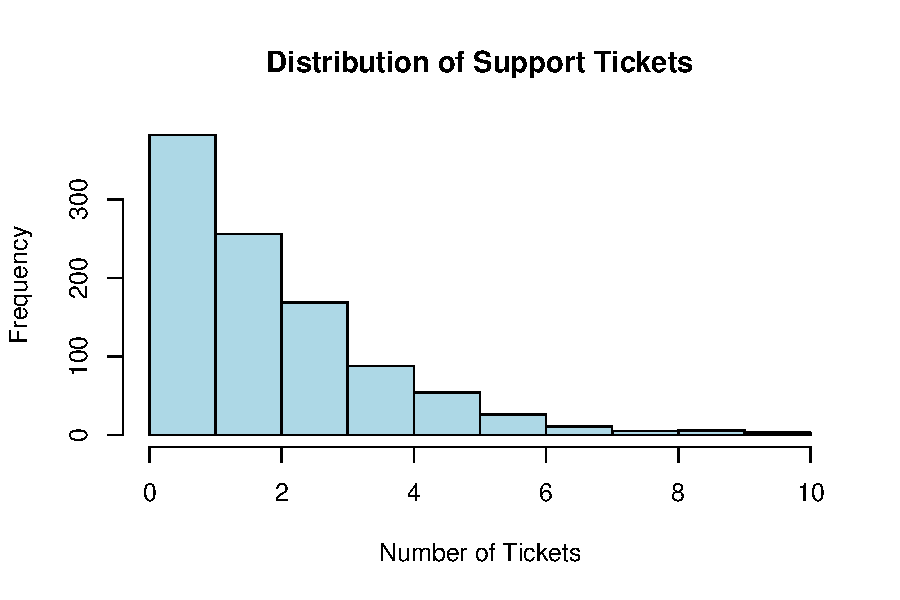
\includegraphics{PROJECT_Final_files/figure-latex/unnamed-chunk-2-1.pdf}

\begin{Shaded}
\begin{Highlighting}[]
\FunctionTok{hist}\NormalTok{(customer.data}\SpecialCharTok{$}\NormalTok{DataUsage\_GB, }
     \AttributeTok{main =} \StringTok{"Distribution of Data Usage"}\NormalTok{,}
     \AttributeTok{xlab =} \StringTok{"GB of Data Used"}\NormalTok{,}
     \AttributeTok{col =} \StringTok{"lightgreen"}\NormalTok{)}
\end{Highlighting}
\end{Shaded}

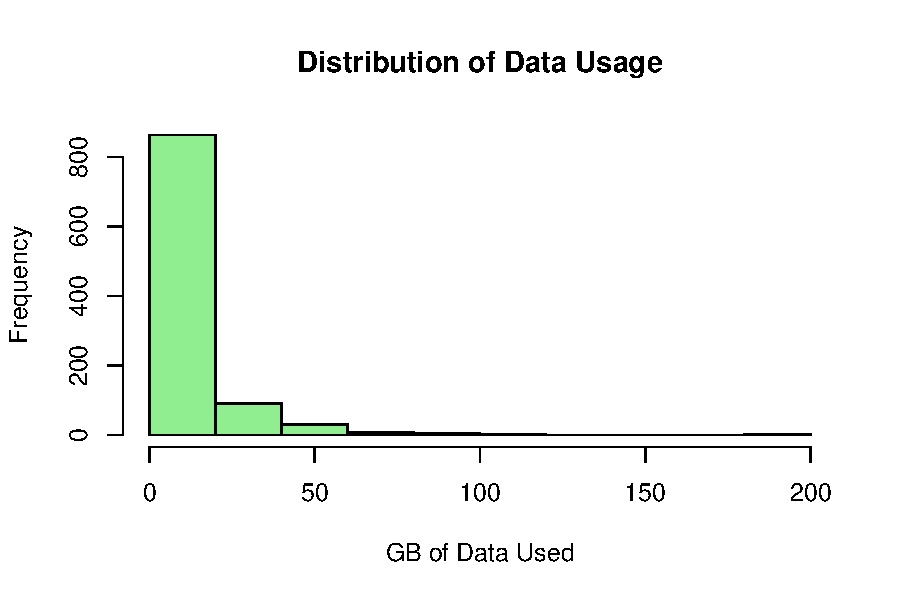
\includegraphics{PROJECT_Final_files/figure-latex/unnamed-chunk-2-2.pdf}

\hfill\break

\textbf{Churn Rate}: 13.4\% of customers churned, highlighting a notable
retention concern in South Africa's highly competitive telecom sector.

\textbf{Age (Mean: 37.97)}: The customer base spans young to middle-aged
adults. Younger users may be more likely to churn due to price
sensitivity or appealing offers from competitors.

\textbf{ContractDuration\_Months (Mean: 15.25, Max: 36)}: While many
customers have medium-term contracts, a segment is on short-term or
month-to-month plans posing a higher churn risk.

\textbf{DataUsage\_GB (Mean: 10.4, Max: 185.8)}: The data is
right-skewed, with a few high-usage customers. Most users consume low to
moderate data, likely due to affordability challenges, especially in
rural regions.

\textbf{SupportTickets (Mean: 2.25, Max: 10)}: Right-skewed distribution
indicates that most users log few support issues, but a small group with
frequent complaints may be at greater risk of churn.

\textbf{SatisfactionScore (Mean: 6.21)}: Average satisfaction is
moderate. Customers with scores below 5 are likely dissatisfied and more
prone to churn.

\textbf{UsageFrequency (Mean: 8.93, Max: 28)}: Indicates moderate
service usage. Higher interaction may reflect greater dependency on
ConnectZA's offerings.

\textbf{SubscriptionTier}: Majority of customers are on Basic (414) or
Standard (440) plans, reflecting a price-sensitive market. These
segments may be more vulnerable to switching for better value.

\textbf{Skewed Variables}: SupportTickets and DataUsage\_GB are
right-skewed and, I used log-transformation to normalize distributions
for modeling.

\hfill\break

\begin{Shaded}
\begin{Highlighting}[]
\CommentTok{\#Churn and SubscriptionTier }

\FunctionTok{ggplot}\NormalTok{(customer.data, }\FunctionTok{aes}\NormalTok{(}\AttributeTok{x =}\NormalTok{ SubscriptionTier, }\AttributeTok{fill =} \FunctionTok{factor}\NormalTok{(Churn))) }\SpecialCharTok{+}
  \FunctionTok{geom\_bar}\NormalTok{(}\AttributeTok{position =} \StringTok{"fill"}\NormalTok{) }\SpecialCharTok{+}
  \FunctionTok{labs}\NormalTok{(}
    \AttributeTok{title =} \StringTok{"Proportion of Churn by Subscription Tier"}\NormalTok{,}
    \AttributeTok{x =} \StringTok{"Tier"}\NormalTok{, }
    \AttributeTok{y =} \StringTok{"Proportion"}\NormalTok{,}
    \AttributeTok{fill =} \StringTok{"Churn Status"}
\NormalTok{  ) }\SpecialCharTok{+}
  \FunctionTok{scale\_fill\_manual}\NormalTok{(}\AttributeTok{values =} \FunctionTok{c}\NormalTok{(}\StringTok{"grey"}\NormalTok{, }\StringTok{"brown"}\NormalTok{), }\AttributeTok{labels =} \FunctionTok{c}\NormalTok{(}\StringTok{"Retained"}\NormalTok{, }\StringTok{"Churned"}\NormalTok{)) }\SpecialCharTok{+}
  \FunctionTok{theme\_minimal}\NormalTok{()}
\end{Highlighting}
\end{Shaded}

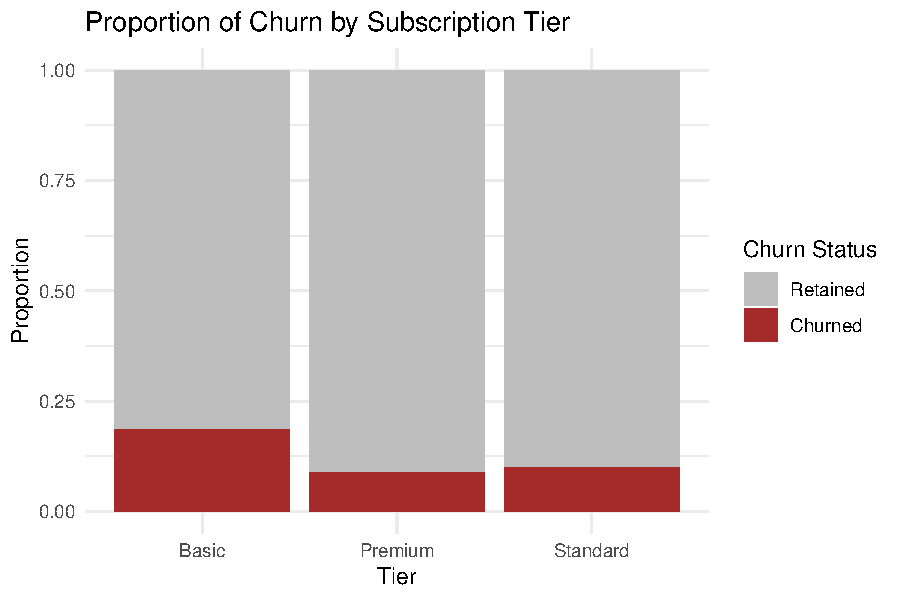
\includegraphics{PROJECT_Final_files/figure-latex/unnamed-chunk-3-1.pdf}

\hfill\break
Basic tier likely shows higher churn. Premium customers often show lower
churn due to better service value. ConnectZA should offer discounts or
bundled services to retain Basic tier customers\\

\begin{Shaded}
\begin{Highlighting}[]
\CommentTok{\#Churn vs SatisfactionScore }
\FunctionTok{ggplot}\NormalTok{(customer.data, }\FunctionTok{aes}\NormalTok{(}\AttributeTok{x =} \FunctionTok{as.factor}\NormalTok{(Churn), }\AttributeTok{y =}\NormalTok{ SatisfactionScore,}
                          \AttributeTok{fill =} \FunctionTok{as.factor}\NormalTok{(Churn))) }\SpecialCharTok{+}  \FunctionTok{geom\_boxplot}\NormalTok{() }\SpecialCharTok{+}
       \FunctionTok{labs}\NormalTok{(}\AttributeTok{x =} \StringTok{"Churn (0 = Stayed, 1 = Churned)"}\NormalTok{, }
       \AttributeTok{y =} \StringTok{"Satisfaction Score"}\NormalTok{, }
       \AttributeTok{title =} \StringTok{"Box Plot of Satisfaction Score by Churn Status"}\NormalTok{,}
       \AttributeTok{fill =} \StringTok{"Churn"}\NormalTok{) }\SpecialCharTok{+} \FunctionTok{scale\_fill\_manual}\NormalTok{(}\AttributeTok{values =} \FunctionTok{c}\NormalTok{(}\StringTok{"grey"}\NormalTok{,}\StringTok{"brown"}\NormalTok{))}\SpecialCharTok{+}
  \FunctionTok{theme\_minimal}\NormalTok{()}
\end{Highlighting}
\end{Shaded}

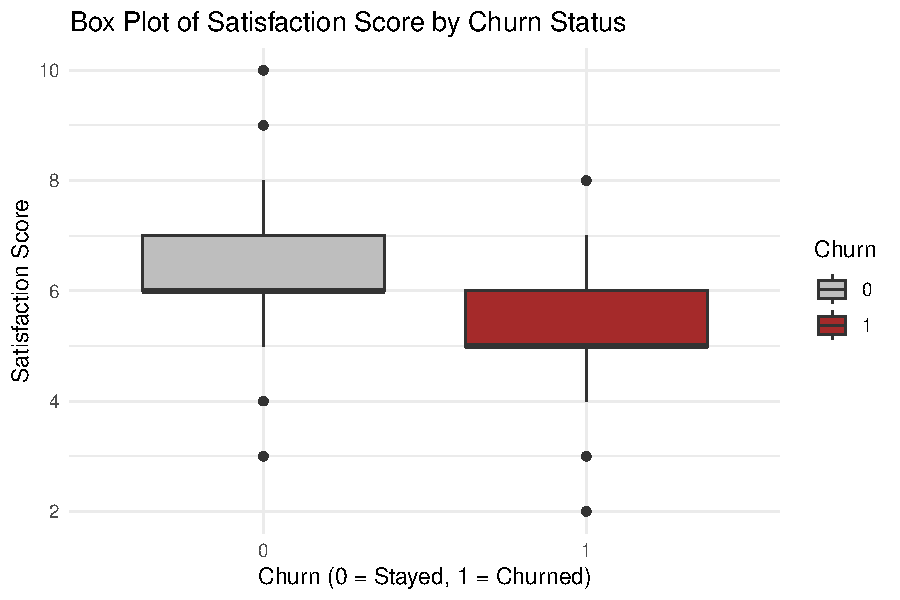
\includegraphics{PROJECT_Final_files/figure-latex/unnamed-chunk-4-1.pdf}

\hfill\break
Sharp increase in churn for scores below 5. Indicates dissatisfaction as
a key churn driver. This supports the idea that customer satisfaction is
closely linked to churn. ConnectZA should focus on improving
satisfaction especially among those scoring below 5 to help reduce
churn. ConnectZA should maybe investigate network coverage or support
quality in rural areas to boost satisfaction and reduce churn.\\

\begin{Shaded}
\begin{Highlighting}[]
\CommentTok{\# Churn vs contractDuration}
\FunctionTok{ggplot}\NormalTok{(customer.data, }\FunctionTok{aes}\NormalTok{(}\AttributeTok{x =} \FunctionTok{as.factor}\NormalTok{(Churn), }\AttributeTok{y =}\NormalTok{ ContractDuration\_Months, }\AttributeTok{fill =} \FunctionTok{as.factor}\NormalTok{(Churn))) }\SpecialCharTok{+}
  \FunctionTok{geom\_boxplot}\NormalTok{() }\SpecialCharTok{+}
  \FunctionTok{labs}\NormalTok{(}\AttributeTok{x =} \StringTok{"Churn (0 = Stayed, 1 = Churned)"}\NormalTok{, }
       \AttributeTok{y =} \StringTok{"Contract Duration (Months)"}\NormalTok{, }
       \AttributeTok{title =} \StringTok{"Box Plot of Contract Duration  by Churn Status"}\NormalTok{,}
       \AttributeTok{fill =} \StringTok{"Churn"}\NormalTok{) }\SpecialCharTok{+} \FunctionTok{scale\_fill\_manual}\NormalTok{(}\AttributeTok{values =} \FunctionTok{c}\NormalTok{(}\StringTok{"grey"}\NormalTok{,}\StringTok{"brown"}\NormalTok{))}\SpecialCharTok{+}
  \FunctionTok{theme\_minimal}\NormalTok{()}
\end{Highlighting}
\end{Shaded}

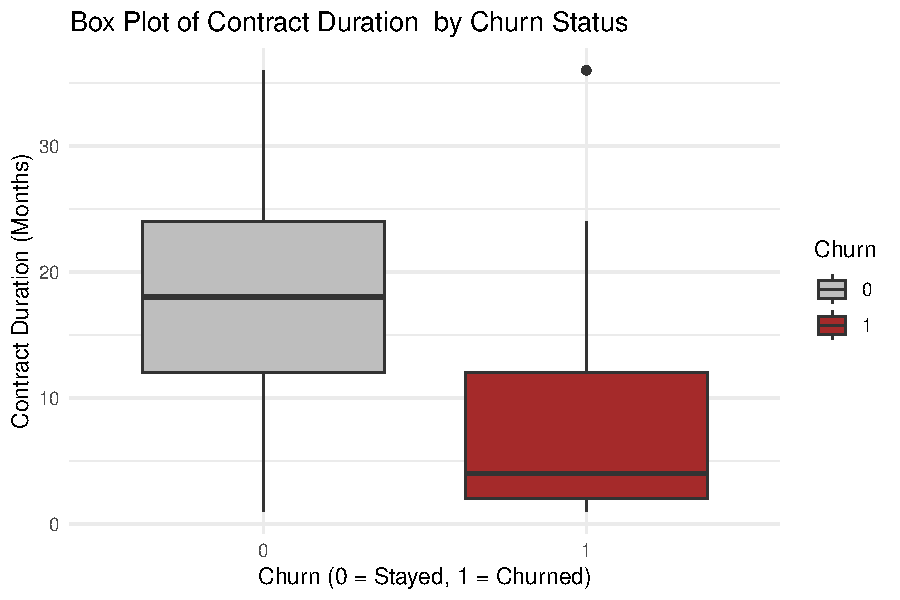
\includegraphics{PROJECT_Final_files/figure-latex/unnamed-chunk-5-1.pdf}

\hfill\break
This box plot shows how long customers' contracts are depending on
whether they stayed or left. Churned customers (Churn = 1) usually have
shorter contracts. The median contract length is higher for those who
stayed.Some customers with very short contracts are especially likely to
churn maybe they're on month to month plans Customers nearing the end of
their contracts are more likely to churn. ConnectZA could target them
with renewal offers before they consider switching to a competitor and
maybe offer loyalty bonuses or data bundles to encourage longer
contracts.\\

\begin{Shaded}
\begin{Highlighting}[]
\CommentTok{\#we want to select numerical variables }
\NormalTok{num\_vars }\OtherTok{\textless{}{-}}\NormalTok{ customer.data[, }\FunctionTok{sapply}\NormalTok{(customer.data, is.numeric)]}

\CommentTok{\#Calaculate correlation matrix}
\NormalTok{cor\_matrix }\OtherTok{\textless{}{-}} \FunctionTok{cor}\NormalTok{(num\_vars)}
\NormalTok{cor\_matrix}
\end{Highlighting}
\end{Shaded}

\begin{verbatim}
##                                   Age ContractDuration_Months DataUsage_GB
## Age                      1.0000000000           -0.0006085568   0.02683444
## ContractDuration_Months -0.0006085568            1.0000000000   0.04239383
## DataUsage_GB             0.0268344426            0.0423938345   1.00000000
## UsageFrequency           0.0325176696           -0.0019986617   0.41496826
## SupportTickets           0.0340223367           -0.3377949755   0.03090526
## SatisfactionScore       -0.0084957160            0.3450512746  -0.02120900
## Churn                   -0.0235741258           -0.3390109130  -0.02154626
##                         UsageFrequency SupportTickets SatisfactionScore
## Age                        0.032517670     0.03402234      -0.008495716
## ContractDuration_Months   -0.001998662    -0.33779498       0.345051275
## DataUsage_GB               0.414968260     0.03090526      -0.021208996
## UsageFrequency             1.000000000     0.03628899       0.034302923
## SupportTickets             0.036288988     1.00000000      -0.315595120
## SatisfactionScore          0.034302923    -0.31559512       1.000000000
## Churn                     -0.125266407     0.43440831      -0.297414544
##                               Churn
## Age                     -0.02357413
## ContractDuration_Months -0.33901091
## DataUsage_GB            -0.02154626
## UsageFrequency          -0.12526641
## SupportTickets           0.43440831
## SatisfactionScore       -0.29741454
## Churn                    1.00000000
\end{verbatim}

\begin{Shaded}
\begin{Highlighting}[]
\CommentTok{\# Visualize}
\FunctionTok{corrplot}\NormalTok{(cor\_matrix, }\AttributeTok{method =} \StringTok{"color"}\NormalTok{, }\AttributeTok{tl.cex =} \FloatTok{0.8}\NormalTok{)}
\end{Highlighting}
\end{Shaded}

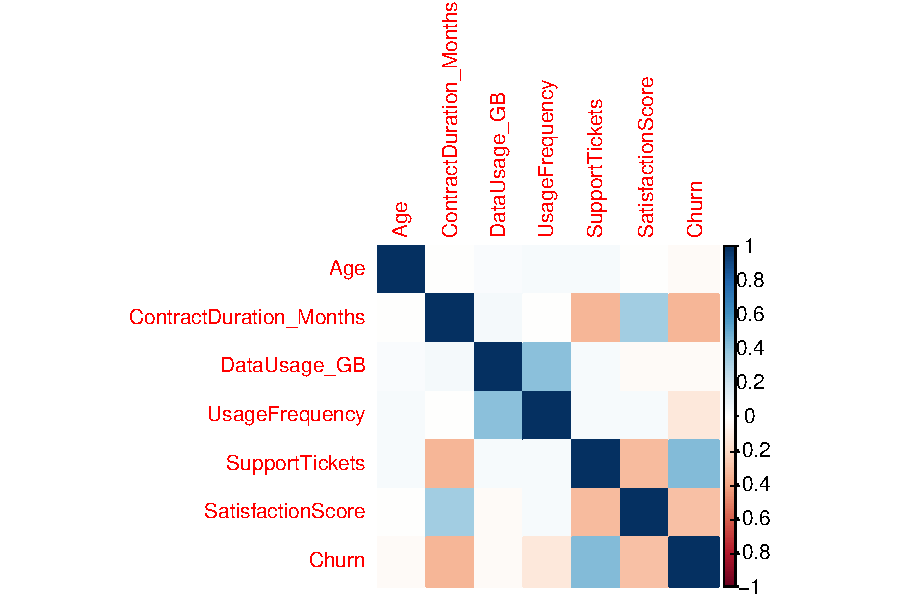
\includegraphics{PROJECT_Final_files/figure-latex/unnamed-chunk-6-1.pdf}

\hfill\break
The correlation between UsageFrequency and SatisfactionScore is weak
(0.034), indicating they capture distinct aspects of customer behavior
(engagement vs.~experience quality). Both should be included in models
to cover different churn drivers. Stronger correlations include
SupportTickets and Churn (0.434), suggesting service issues
significantly increase churn likelihood, and SatisfactionScore and Churn
(-0.297), confirming higher satisfaction reduces churn. No correlations
exceed 0.7, reducing multicollinearity concerns for modeling. ConnectZA
can use these insights to prioritize support resolution and satisfaction
improvements in modeling and retention strategies.\\

\begin{Shaded}
\begin{Highlighting}[]
\CommentTok{\#Transforming the Skewed data : Log transformation}
\NormalTok{customer.data}\SpecialCharTok{$}\NormalTok{SupportTickets }\OtherTok{\textless{}{-}} \FunctionTok{log}\NormalTok{(customer.data}\SpecialCharTok{$}\NormalTok{SupportTickets }\SpecialCharTok{+} \DecValTok{1}\NormalTok{ ) }\CommentTok{\# we add the1 to avoid log(0)}
\NormalTok{customer.data}\SpecialCharTok{$}\NormalTok{DataUsage\_GB}\OtherTok{\textless{}{-}} \FunctionTok{log}\NormalTok{(customer.data}\SpecialCharTok{$}\NormalTok{DataUsage\_GB }\SpecialCharTok{+}\DecValTok{1}\NormalTok{ )}

\CommentTok{\# Verify transformation}
\FunctionTok{hist}\NormalTok{(customer.data}\SpecialCharTok{$}\NormalTok{SupportTickets, }\AttributeTok{main =} \StringTok{"Log{-}Transformed Support Tickets"}\NormalTok{, }\AttributeTok{xlab =} \StringTok{"Log(Number of Tickets)"}\NormalTok{, }\AttributeTok{col =} \StringTok{"lightblue"}\NormalTok{)}
\end{Highlighting}
\end{Shaded}

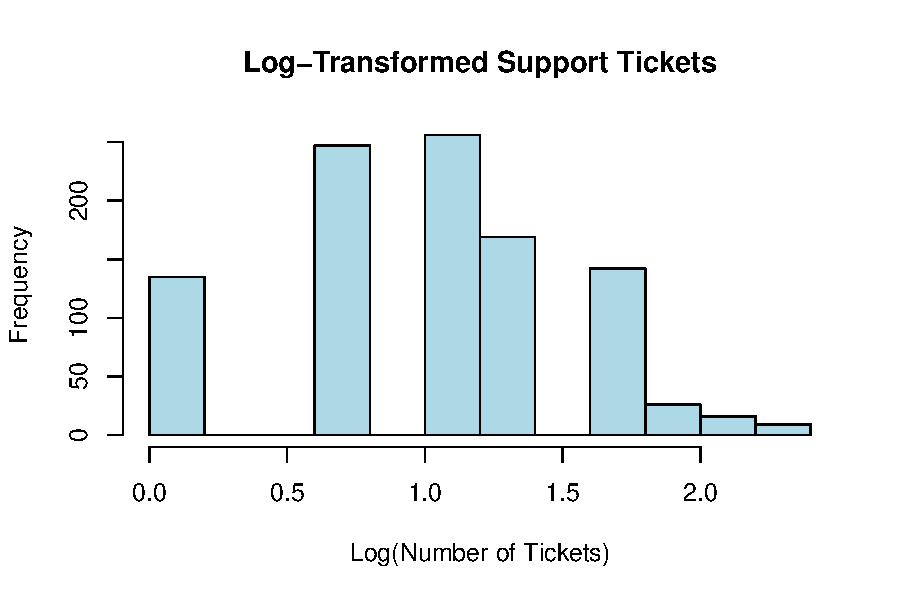
\includegraphics{PROJECT_Final_files/figure-latex/unnamed-chunk-7-1.pdf}

\begin{Shaded}
\begin{Highlighting}[]
\FunctionTok{hist}\NormalTok{(customer.data}\SpecialCharTok{$}\NormalTok{DataUsage\_GB, }\AttributeTok{main =} \StringTok{"Log{-}Transformed Data Usage"}\NormalTok{, }\AttributeTok{xlab =} \StringTok{"Log(GB of Data Used)"}\NormalTok{, }\AttributeTok{col =} \StringTok{"lightgreen"}\NormalTok{)}
\end{Highlighting}
\end{Shaded}

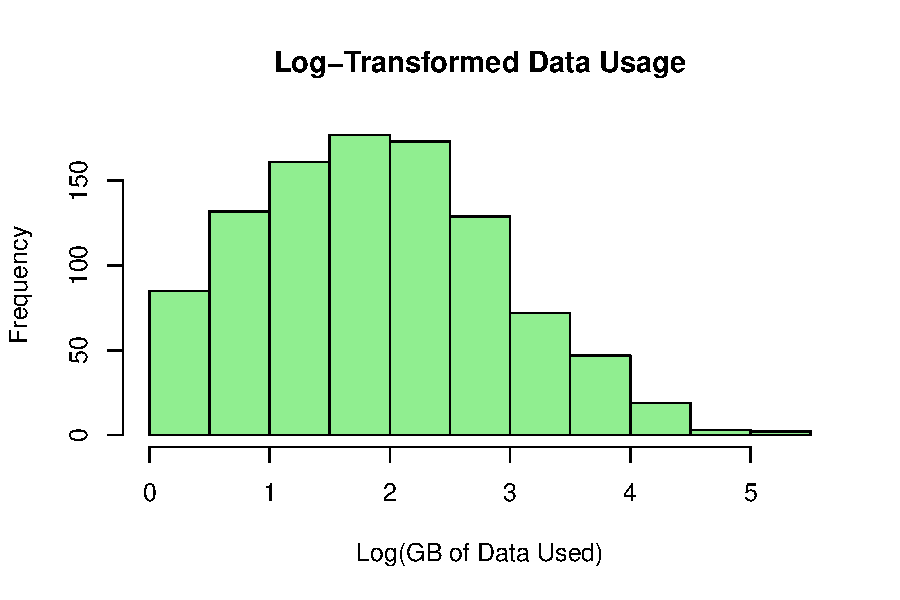
\includegraphics{PROJECT_Final_files/figure-latex/unnamed-chunk-7-2.pdf}

\begin{Shaded}
\begin{Highlighting}[]
\CommentTok{\#Partitioning the data into Train{-}test split(70\textbackslash{}30 split).}
\FunctionTok{set.seed}\NormalTok{(}\DecValTok{42}\NormalTok{)}
\NormalTok{n }\OtherTok{\textless{}{-}} \FunctionTok{nrow}\NormalTok{(customer.data)}
\NormalTok{p }\OtherTok{\textless{}{-}} \FloatTok{0.7}

\NormalTok{training.indices }\OtherTok{\textless{}{-}} \FunctionTok{sample}\NormalTok{(}\FunctionTok{seq}\NormalTok{(}\DecValTok{1}\NormalTok{, n), }\AttributeTok{size =}\NormalTok{ n }\SpecialCharTok{*}\NormalTok{ p)}
\NormalTok{training.set }\OtherTok{\textless{}{-}}\NormalTok{ customer.data[training.indices, ]}
\NormalTok{test.set }\OtherTok{\textless{}{-}}\NormalTok{ customer.data[}\SpecialCharTok{{-}}\NormalTok{training.indices, ]}
\end{Highlighting}
\end{Shaded}

\hfill\break
\textbf{Decisions:}\\
\textbf{Log Transformation:} SupportTickets and DataUsage\_GB exhibited
substantial right skew. Applying a log transformation reduces skewness
and stabilises variance. This preprocessing step improves the
suitability of these predictors for linear classification methods such
as LPM and LDA, which rely on assumptions of linearity and, in the case
of LDA, approximate normality.\\
\textbf{Train-Test Split:} A 70-30 split was implemented using
set.seed(42) to ensure reproducibility. This allocation offers a
balanced approach, providing sufficient data for model training while
preserving enough cases to robustly evaluate predictive performance on
the test set.\\
\textbf{Ethical Consideration:} Churn prediction can unintentionally
reinforce socioeconomic bias. For example, rural or low-income customers
may show lower DataUsage\_GB due to poor coverage, not disinterest,
risking exclusion from retention efforts. ConnectZA should audit models
for demographic bias and offer subsidised data plans to support
equitable retention.\\

\hypertarget{linear-probability-model}{%
\subsection{LINEAR PROBABILITY MODEL}\label{linear-probability-model}}

\begin{Shaded}
\begin{Highlighting}[]
\CommentTok{\# Convert SubscriptionTier to factor}
\NormalTok{customer.data}\SpecialCharTok{$}\NormalTok{SubscriptionTier }\OtherTok{\textless{}{-}} \FunctionTok{as.factor}\NormalTok{(customer.data}\SpecialCharTok{$}\NormalTok{SubscriptionTier)}
\FunctionTok{summary}\NormalTok{(customer.data}\SpecialCharTok{$}\NormalTok{SubscriptionTier)}
\end{Highlighting}
\end{Shaded}

\begin{verbatim}
##    Basic  Premium Standard 
##      414      146      440
\end{verbatim}

\begin{Shaded}
\begin{Highlighting}[]
\CommentTok{\#LPM }
\NormalTok{my.lpm }\OtherTok{\textless{}{-}} \FunctionTok{lm}\NormalTok{(Churn }\SpecialCharTok{\textasciitilde{}}\NormalTok{ ., }\AttributeTok{data =}\NormalTok{ training.set)}
\FunctionTok{summary}\NormalTok{(my.lpm)}
\end{Highlighting}
\end{Shaded}

\begin{verbatim}
## 
## Call:
## lm(formula = Churn ~ ., data = training.set)
## 
## Residuals:
##      Min       1Q   Median       3Q      Max 
## -0.51624 -0.19551 -0.08272  0.08217  1.00476 
## 
## Coefficients:
##                            Estimate Std. Error t value Pr(>|t|)    
## (Intercept)               0.4072486  0.0861450   4.727 2.76e-06 ***
## Age                      -0.0005872  0.0009996  -0.587  0.55709    
## SubscriptionTierPremium  -0.0857971  0.0607655  -1.412  0.15842    
## SubscriptionTierStandard -0.0839462  0.0311520  -2.695  0.00722 ** 
## ContractDuration_Months  -0.0076237  0.0012077  -6.313 4.90e-10 ***
## DataUsage_GB              0.0337373  0.0130107   2.593  0.00971 ** 
## UsageFrequency           -0.0073835  0.0037582  -1.965  0.04985 *  
## SupportTickets            0.1758261  0.0220048   7.990 5.64e-15 ***
## SatisfactionScore        -0.0418966  0.0105277  -3.980 7.63e-05 ***
## ---
## Signif. codes:  0 '***' 0.001 '**' 0.01 '*' 0.05 '.' 0.1 ' ' 1
## 
## Residual standard error: 0.3003 on 691 degrees of freedom
## Multiple R-squared:  0.2667, Adjusted R-squared:  0.2582 
## F-statistic: 31.42 on 8 and 691 DF,  p-value: < 2.2e-16
\end{verbatim}

\hfill\break
The R-squared value is 0.2667 which tell us that about 27\% of the
variation in churn can be explained. Whilst other factors may also drive
churn. The F-statistics is 31.42 and has a very small P-value (less than
0.05) which tells us that the model is statistically significant,
therefore at least one of the predictor variables is meaningfully
related to churn.\\

\begin{Shaded}
\begin{Highlighting}[]
\CommentTok{\# Extract significant predictors (p \textless{} 0.05)}
\FunctionTok{summary}\NormalTok{(my.lpm)}\SpecialCharTok{$}\NormalTok{coefficients[}\FunctionTok{summary}\NormalTok{(my.lpm)}\SpecialCharTok{$}\NormalTok{coefficients[, }\DecValTok{4}\NormalTok{] }\SpecialCharTok{\textless{}} \FloatTok{0.05}\NormalTok{, ]}
\end{Highlighting}
\end{Shaded}

\begin{verbatim}
##                              Estimate  Std. Error   t value     Pr(>|t|)
## (Intercept)               0.407248600 0.086145023  4.727477 2.755983e-06
## SubscriptionTierStandard -0.083946182 0.031151966 -2.694731 7.215731e-03
## ContractDuration_Months  -0.007623719 0.001207666 -6.312768 4.900816e-10
## DataUsage_GB              0.033737281 0.013010692  2.593043 9.714401e-03
## UsageFrequency           -0.007383548 0.003758193 -1.964654 4.985466e-02
## SupportTickets            0.175826107 0.022004806  7.990350 5.643306e-15
## SatisfactionScore        -0.041896576 0.010527653 -3.979669 7.630582e-05
\end{verbatim}

\textbf{Significant Predictors}\\
\textbf{ContractDuration\_Months:} A coefficient of -0.0076 tells us
that an additional month to a customers contract reduces their churn
probability by around 0.76\%. Then it clear that longer contracts help
keep customers. ConnectZA could introduces maybe loyalty bonuses to
customers to encourage longer commitments from them. ConnectZa should
maybe offer discounted renewals for customers with contracts under 6
months\\
\textbf{SupportTickets:} Each additional support ticket raised increases
the churn probability by 17.58\%. Poor service experiences (reflected in
support tickets) drastically increase churn risk. ConnectZA should
prioritize resolving issues for customers with at most 2 tickets\\

\begin{Shaded}
\begin{Highlighting}[]
\NormalTok{yhat }\OtherTok{\textless{}{-}} \FunctionTok{predict}\NormalTok{(my.lpm, }\AttributeTok{newdata =}\NormalTok{ test.set)}
\NormalTok{y }\OtherTok{\textless{}{-}}\NormalTok{ test.set}\SpecialCharTok{$}\NormalTok{Churn}

\NormalTok{Prediction\_outside }\OtherTok{\textless{}{-}} \FunctionTok{sum}\NormalTok{(yhat }\SpecialCharTok{\textless{}} \DecValTok{0} \SpecialCharTok{|}\NormalTok{ yhat }\SpecialCharTok{\textgreater{}} \DecValTok{1}\NormalTok{)}
\NormalTok{Prediction\_outside}
\end{Highlighting}
\end{Shaded}

\begin{verbatim}
## [1] 73
\end{verbatim}

\begin{Shaded}
\begin{Highlighting}[]
\NormalTok{Prediction\_outside\_class }\OtherTok{\textless{}{-}} \FunctionTok{ifelse}\NormalTok{(yhat }\SpecialCharTok{\textgreater{}} \FloatTok{0.5}\NormalTok{, }\DecValTok{1}\NormalTok{, }\DecValTok{0}\NormalTok{)}
\NormalTok{conf\_matrix }\OtherTok{\textless{}{-}} \FunctionTok{table}\NormalTok{(}\AttributeTok{Predicted =}\NormalTok{ Prediction\_outside\_class, }\AttributeTok{Actual =}\NormalTok{ test.set}\SpecialCharTok{$}\NormalTok{Churn)}
\NormalTok{conf\_matrix}
\end{Highlighting}
\end{Shaded}

\begin{verbatim}
##          Actual
## Predicted   0   1
##         0 264  33
##         1   1   2
\end{verbatim}

\begin{Shaded}
\begin{Highlighting}[]
\NormalTok{accuracy }\OtherTok{\textless{}{-}}\NormalTok{ (conf\_matrix[}\DecValTok{1}\NormalTok{,}\DecValTok{1}\NormalTok{] }\SpecialCharTok{+}\NormalTok{ conf\_matrix[}\DecValTok{2}\NormalTok{,}\DecValTok{2}\NormalTok{]) }\SpecialCharTok{/} \FunctionTok{sum}\NormalTok{(conf\_matrix)}
\NormalTok{sensitivity }\OtherTok{\textless{}{-}}\NormalTok{ conf\_matrix[}\DecValTok{2}\NormalTok{,}\DecValTok{2}\NormalTok{] }\SpecialCharTok{/} \FunctionTok{sum}\NormalTok{(conf\_matrix[,}\DecValTok{2}\NormalTok{])}
\NormalTok{specificity }\OtherTok{\textless{}{-}}\NormalTok{ conf\_matrix[}\DecValTok{1}\NormalTok{,}\DecValTok{1}\NormalTok{] }\SpecialCharTok{/} \FunctionTok{sum}\NormalTok{(conf\_matrix[,}\DecValTok{1}\NormalTok{])}

\NormalTok{accuracy}
\end{Highlighting}
\end{Shaded}

\begin{verbatim}
## [1] 0.8866667
\end{verbatim}

\begin{Shaded}
\begin{Highlighting}[]
\NormalTok{sensitivity}
\end{Highlighting}
\end{Shaded}

\begin{verbatim}
## [1] 0.05714286
\end{verbatim}

\begin{Shaded}
\begin{Highlighting}[]
\NormalTok{specificity}
\end{Highlighting}
\end{Shaded}

\begin{verbatim}
## [1] 0.9962264
\end{verbatim}

\hfill\break
\textbf{THE LIMITATIONS OF THE LINEAR PROBABILITY MODEL}\\
The Linear Probability Model (LPM) has several mathematical and
practical limitations that reduce its effectiveness for ConnectZA's
churn prediction in the South African telecommunications market:

\textbf{Predictions Outside Valid Probability Range}: The LPM can
produce predicted probabilities less than 0 or greater than 1, which are
uninterpretable as probabilities. In the test set, 73 out of 300
predictions (24.3\%) fall outside {[}0,1{]}, such as a predicted churn
probability of 1.65 for a rural customer with low DataUsage\_GB. This
can lead ConnectZA to misclassify low-risk rural customers as high-risk,
wasting retention resources (e.g., R5M annually on misdirected loyalty
offers) and undermining the ``Hlala Nathi'' programme's effectiveness.

\textbf{Inability to Capture Non-Linear Relationships}: The LPM assumes
a linear relationship between predictors and churn probability, which
fails to model complex patterns, such as the sharp increase in churn
risk for customers with high SupportTickets.This limitation may cause
ConnectZA to overlook key churn drivers like poor network quality in
urban areas, risking the loss of thousands of customers.\\

\hypertarget{logistic-regression}{%
\subsection{LOGISTIC REGRESSION}\label{logistic-regression}}

\begin{Shaded}
\begin{Highlighting}[]
\CommentTok{\# Fit logistic regression}
\NormalTok{MLR }\OtherTok{\textless{}{-}} \FunctionTok{glm}\NormalTok{(Churn }\SpecialCharTok{\textasciitilde{}}\NormalTok{ ., }\AttributeTok{data =}\NormalTok{ training.set, }\AttributeTok{family =}\NormalTok{ binomial)}
\FunctionTok{summary}\NormalTok{(MLR)}
\end{Highlighting}
\end{Shaded}

\begin{verbatim}
## 
## Call:
## glm(formula = Churn ~ ., family = binomial, data = training.set)
## 
## Coefficients:
##                          Estimate Std. Error z value Pr(>|z|)    
## (Intercept)               1.69557    1.25328   1.353  0.17609    
## Age                      -0.01504    0.01248  -1.205  0.22806    
## SubscriptionTierPremium  -1.03633    0.73286  -1.414  0.15733    
## SubscriptionTierStandard -1.04455    0.38768  -2.694  0.00705 ** 
## ContractDuration_Months  -0.13084    0.02251  -5.812 6.18e-09 ***
## DataUsage_GB              0.43349    0.17265   2.511  0.01205 *  
## UsageFrequency           -0.11151    0.05009  -2.226  0.02600 *  
## SupportTickets            1.93463    0.34690   5.577 2.45e-08 ***
## SatisfactionScore        -0.58713    0.14500  -4.049 5.14e-05 ***
## ---
## Signif. codes:  0 '***' 0.001 '**' 0.01 '*' 0.05 '.' 0.1 ' ' 1
## 
## (Dispersion parameter for binomial family taken to be 1)
## 
##     Null deviance: 570.57  on 699  degrees of freedom
## Residual deviance: 339.30  on 691  degrees of freedom
## AIC: 357.3
## 
## Number of Fisher Scoring iterations: 7
\end{verbatim}

\hfill\break
The above Logistic Regression Model gives a better fit than the Linear
Probability Model and avoids invalid predictions since it all the
predicted values from this model will fall within the valid probability
range {[}0,1{]}. which makes its appropriate for real world business
decision. The areas in which the model highlights that Customer
satisfaction (SatistfactionScore), Contract Duration
(ContractDuration\_Months) and, Support Experience (SupportTickets) are
areas that ConnectZA should focus on to reduce Churn. The logistic
regression model shows significant predictors like SupportTickets
(coefficient = 1.93463, p \textless{} 0.001), indicating that each
additional log-transformed ticket increases the log-odds of churn by
1.93, and SatisfactionScore (coefficient = -0.58713, p \textless{}
0.001), showing that higher satisfaction reduces churn likelihood\\

\begin{Shaded}
\begin{Highlighting}[]
\CommentTok{\#Calculate odds ratios}
\NormalTok{odds.ratios }\OtherTok{\textless{}{-}} \FunctionTok{exp}\NormalTok{(}\FunctionTok{coef}\NormalTok{(MLR))}
\NormalTok{odds.table }\OtherTok{\textless{}{-}} \FunctionTok{data.frame}\NormalTok{(}\AttributeTok{OddsRatio =}\NormalTok{ odds.ratios)}
\NormalTok{odds.table}
\end{Highlighting}
\end{Shaded}

\begin{verbatim}
##                          OddsRatio
## (Intercept)              5.4497243
## Age                      0.9850726
## SubscriptionTierPremium  0.3547544
## SubscriptionTierStandard 0.3518499
## ContractDuration_Months  0.8773553
## DataUsage_GB             1.5426318
## UsageFrequency           0.8944830
## SupportTickets           6.9214821
## SatisfactionScore        0.5559205
\end{verbatim}

\hfill\break
The odds ratio for SupportTickets is 6.92, which means that for every
extra support ticket a customer logs, their chances of churning are
almost seven times higher. This shows that customers who face frequent
problems are much more likely to leave. On the other hand, the odds
ratio for SatisfactionScore is 0.56, so if a customer's satisfaction
score goes up by just one point, their likelihood of churning drops by
about 44\%. This proves how important it is for ConnectZA to keep
customers happy and handle support issues properly to reduce
churn.Unlike LPM's probability changes, logistic regression's odds
ratios (e.g., 6.92 for SupportTickets) show multiplicative effects on
churn odds, providing clearer insights for targeting high-risk customers
with improved support solutions.\\

\begin{Shaded}
\begin{Highlighting}[]
\CommentTok{\# Predict on test set}
\NormalTok{yhat.predicted }\OtherTok{\textless{}{-}} \FunctionTok{predict}\NormalTok{(MLR, }\AttributeTok{newdata =}\NormalTok{ test.set, }\AttributeTok{type =} \StringTok{"response"}\NormalTok{)}
\NormalTok{yhat.pred.class }\OtherTok{\textless{}{-}} \FunctionTok{ifelse}\NormalTok{(yhat.predicted }\SpecialCharTok{\textgreater{}} \FloatTok{0.5}\NormalTok{, }\DecValTok{1}\NormalTok{, }\DecValTok{0}\NormalTok{)}

\CommentTok{\# Confusion matrix}
\NormalTok{conf\_matrix\_mrl }\OtherTok{\textless{}{-}} \FunctionTok{table}\NormalTok{(}\AttributeTok{Predicted =}\NormalTok{ yhat.pred.class , }\AttributeTok{Actual =}\NormalTok{ test.set}\SpecialCharTok{$}\NormalTok{Churn )}
\NormalTok{conf\_matrix\_mrl}
\end{Highlighting}
\end{Shaded}

\begin{verbatim}
##          Actual
## Predicted   0   1
##         0 256  23
##         1   9  12
\end{verbatim}

\begin{Shaded}
\begin{Highlighting}[]
\CommentTok{\# Performance metrics}
\NormalTok{accuracy }\OtherTok{\textless{}{-}}\NormalTok{ (conf\_matrix\_mrl[}\DecValTok{1}\NormalTok{,}\DecValTok{1}\NormalTok{] }\SpecialCharTok{+}\NormalTok{ conf\_matrix\_mrl[}\DecValTok{2}\NormalTok{,}\DecValTok{2}\NormalTok{]) }\SpecialCharTok{/} \FunctionTok{sum}\NormalTok{(conf\_matrix\_mrl)}
\NormalTok{sensitivity }\OtherTok{\textless{}{-}}\NormalTok{ conf\_matrix\_mrl[}\DecValTok{2}\NormalTok{,}\DecValTok{2}\NormalTok{] }\SpecialCharTok{/} \FunctionTok{sum}\NormalTok{(conf\_matrix\_mrl[,}\DecValTok{2}\NormalTok{])}
\NormalTok{specificity }\OtherTok{\textless{}{-}}\NormalTok{ conf\_matrix\_mrl[}\DecValTok{1}\NormalTok{,}\DecValTok{1}\NormalTok{] }\SpecialCharTok{/} \FunctionTok{sum}\NormalTok{(conf\_matrix\_mrl[,}\DecValTok{1}\NormalTok{])}

\NormalTok{accuracy}
\end{Highlighting}
\end{Shaded}

\begin{verbatim}
## [1] 0.8933333
\end{verbatim}

\begin{Shaded}
\begin{Highlighting}[]
\NormalTok{sensitivity}
\end{Highlighting}
\end{Shaded}

\begin{verbatim}
## [1] 0.3428571
\end{verbatim}

\begin{Shaded}
\begin{Highlighting}[]
\NormalTok{specificity}
\end{Highlighting}
\end{Shaded}

\begin{verbatim}
## [1] 0.9660377
\end{verbatim}

\hfill\break
Logistic regression achieves higher specificity (0.343) compared to LPM
(0.057) which ensures better identification of churned customers.This is
critical for ConnectZA's targeted retention efforts.\\

\hypertarget{linear-dicriminant-analysis}{%
\subsection{LINEAR DICRIMINANT
ANALYSIS}\label{linear-dicriminant-analysis}}

\begin{Shaded}
\begin{Highlighting}[]
\CommentTok{\# Fitting my  LDA}
\NormalTok{lda.model }\OtherTok{\textless{}{-}} \FunctionTok{lda}\NormalTok{(Churn}\SpecialCharTok{\textasciitilde{}}\NormalTok{., }\AttributeTok{data =}\NormalTok{ training.set)}
\NormalTok{lda.model}
\end{Highlighting}
\end{Shaded}

\begin{verbatim}
## Call:
## lda(Churn ~ ., data = training.set)
## 
## Prior probabilities of groups:
##         0         1 
## 0.8585714 0.1414286 
## 
## Group means:
##        Age SubscriptionTierPremium SubscriptionTierStandard
## 0 37.93012               0.1464226                0.4808652
## 1 37.39394               0.1010101                0.3131313
##   ContractDuration_Months DataUsage_GB UsageFrequency SupportTickets
## 0               16.605657     1.890290       9.135940      0.9564291
## 1                6.212121     1.893035       7.024242      1.5718290
##   SatisfactionScore
## 0          6.354409
## 1          5.272727
## 
## Coefficients of linear discriminants:
##                                   LD1
## Age                      -0.003804851
## SubscriptionTierPremium  -0.555934611
## SubscriptionTierStandard -0.543941268
## ContractDuration_Months  -0.049398974
## DataUsage_GB              0.218605527
## UsageFrequency           -0.047842750
## SupportTickets            1.139290361
## SatisfactionScore        -0.271474844
\end{verbatim}

\hfill\break
The Linear Discriminant Analysis model shows that customers who churn
tend to have shorter contracts, lower satisfaction scores, and more
support issues compared to those who stay. SatisfactionScore and
ContractDuration\_Months have large negative weights, which shows that
higher satisfaction and longer contracts reduce the chance of churn.
This means ConnectZA should focus on customers with poor support
experiences, low satisfaction, and short contracts as they are the most
at risk.The positive coefficient for SupportTickets (1.139) indicates it
strongly distinguishes churned customers, urging ConnectZA to enhance
support efficiency\\

\begin{Shaded}
\begin{Highlighting}[]
\NormalTok{lda.model.means}\OtherTok{\textless{}{-}}\NormalTok{lda.model}\SpecialCharTok{$}\NormalTok{means}
\NormalTok{lda.model.means}
\end{Highlighting}
\end{Shaded}

\begin{verbatim}
##        Age SubscriptionTierPremium SubscriptionTierStandard
## 0 37.93012               0.1464226                0.4808652
## 1 37.39394               0.1010101                0.3131313
##   ContractDuration_Months DataUsage_GB UsageFrequency SupportTickets
## 0               16.605657     1.890290       9.135940      0.9564291
## 1                6.212121     1.893035       7.024242      1.5718290
##   SatisfactionScore
## 0          6.354409
## 1          5.272727
\end{verbatim}

\hfill\break
\textbf{Group Means:}\\
The group means from the Linear Discriminant Analysis model reveal that
the two most distinguishing variables between churned and non-churned
customers are SupportTickets and ContractDuration\_Months. Customers who
stayed had longer contract duration on average (16.61 months) compared
to those who churned (6.21 months), suggesting that shorter contracts
are associated with a higher risk of churn. It is also visible that
customers with with lesser support response time are unlikely to churn
(0.96) compare to those who got to wait longer for support (1.57). These
findings imply that ConnectZA should improve support response time and
focus on retaining customers whose contracts are nearing expiration.\\

\begin{Shaded}
\begin{Highlighting}[]
\NormalTok{yhat.lda }\OtherTok{\textless{}{-}} \FunctionTok{predict}\NormalTok{(lda.model, }\AttributeTok{newdata=}\NormalTok{test.set)}
\NormalTok{lda.classes }\OtherTok{\textless{}{-}}\NormalTok{ yhat.lda}\SpecialCharTok{$}\NormalTok{class}
\FunctionTok{summary}\NormalTok{(lda.classes)}
\end{Highlighting}
\end{Shaded}

\begin{verbatim}
##   0   1 
## 283  17
\end{verbatim}

\begin{Shaded}
\begin{Highlighting}[]
\NormalTok{conf\_matrix\_lda }\OtherTok{\textless{}{-}} \FunctionTok{table}\NormalTok{(}\AttributeTok{Predicted =}\NormalTok{ lda.classes ,}\AttributeTok{Actual =}\NormalTok{ test.set}\SpecialCharTok{$}\NormalTok{Churn )}
\NormalTok{conf\_matrix\_lda}
\end{Highlighting}
\end{Shaded}

\begin{verbatim}
##          Actual
## Predicted   0   1
##         0 258  25
##         1   7  10
\end{verbatim}

\begin{Shaded}
\begin{Highlighting}[]
\NormalTok{accuracy }\OtherTok{\textless{}{-}}\NormalTok{ (conf\_matrix\_lda[}\DecValTok{1}\NormalTok{,}\DecValTok{1}\NormalTok{] }\SpecialCharTok{+}\NormalTok{ conf\_matrix\_lda[}\DecValTok{2}\NormalTok{,}\DecValTok{2}\NormalTok{]) }\SpecialCharTok{/} \FunctionTok{sum}\NormalTok{(conf\_matrix\_lda)}
\NormalTok{sensitivity }\OtherTok{\textless{}{-}}\NormalTok{ conf\_matrix\_lda[}\DecValTok{2}\NormalTok{,}\DecValTok{2}\NormalTok{] }\SpecialCharTok{/} \FunctionTok{sum}\NormalTok{(conf\_matrix\_lda[,}\DecValTok{2}\NormalTok{])}
\NormalTok{specificity }\OtherTok{\textless{}{-}}\NormalTok{ conf\_matrix\_lda[}\DecValTok{1}\NormalTok{,}\DecValTok{1}\NormalTok{] }\SpecialCharTok{/} \FunctionTok{sum}\NormalTok{(conf\_matrix\_lda[,}\DecValTok{1}\NormalTok{])}

\NormalTok{accuracy}
\end{Highlighting}
\end{Shaded}

\begin{verbatim}
## [1] 0.8933333
\end{verbatim}

\begin{Shaded}
\begin{Highlighting}[]
\NormalTok{sensitivity}
\end{Highlighting}
\end{Shaded}

\begin{verbatim}
## [1] 0.2857143
\end{verbatim}

\begin{Shaded}
\begin{Highlighting}[]
\NormalTok{specificity}
\end{Highlighting}
\end{Shaded}

\begin{verbatim}
## [1] 0.9735849
\end{verbatim}

\hfill\break
In one of the above, the Linear Discriminant Analysis (LDA) model
achieved an accuracy of 89.3\%, sensitivity of 28.6\%, and specificity
of 97.4\%. Compared to the Linear Probability Model , which had a
sensitivity of only 5.7\% and specificity of 99.6\%, LDA demonstrates a
significantly improved ability to identify customers who churn (28.6\%
vs.~5.7\%) while maintaining strong performance in identifying those who
stay. Although LDA's accuracy matches that of logistic regression, its
lower sensitivity makes it less effective at detecting churners.
Additionally, LDA assumes normally distributed predictors and equal
covariance across groups---assumptions that may not hold with skewed
data like SupportTickets or DataUsage\_GB, even after transformation.
Therefore, while LDA offers a more balanced alternative to LPM, logistic
regression remains the more robust and business-appropriate model for
ConnectZA's retention goals.\\

\hypertarget{model-comprasions-and-business-recommendations}{%
\subsection{MODEL COMPRASIONS AND BUSINESS
RECOMMENDATIONS}\label{model-comprasions-and-business-recommendations}}

\begin{Shaded}
\begin{Highlighting}[]
\CommentTok{\# Model Comparison and Recommendation}

\NormalTok{Model.Comparison.Table }\OtherTok{\textless{}{-}} \FunctionTok{data.frame}\NormalTok{(}
  \AttributeTok{Model =} \FunctionTok{c}\NormalTok{(}\StringTok{"Linear Probability Model (LPM)"}\NormalTok{, }
            \StringTok{"Logistic Regression"}\NormalTok{, }
            \StringTok{"Linear Discriminant Analysis (LDA)"}\NormalTok{),}
  \AttributeTok{Accuracy =} \FunctionTok{c}\NormalTok{(}\FloatTok{0.887}\NormalTok{, }\FloatTok{0.893}\NormalTok{, }\FloatTok{0.893}\NormalTok{),}
  \AttributeTok{Sensitivity =} \FunctionTok{c}\NormalTok{(}\FloatTok{0.996}\NormalTok{, }\FloatTok{0.966}\NormalTok{, }\FloatTok{0.974}\NormalTok{),}
  \AttributeTok{Specificity =} \FunctionTok{c}\NormalTok{(}\FloatTok{0.057}\NormalTok{, }\FloatTok{0.343}\NormalTok{, }\FloatTok{0.286}\NormalTok{)}
\NormalTok{)}
\NormalTok{Model.Comparison.Table}
\end{Highlighting}
\end{Shaded}

\begin{verbatim}
##                                Model Accuracy Sensitivity Specificity
## 1     Linear Probability Model (LPM)    0.887       0.996       0.057
## 2                Logistic Regression    0.893       0.966       0.343
## 3 Linear Discriminant Analysis (LDA)    0.893       0.974       0.286
\end{verbatim}

Logistic Regression is the most suitable model for ConnectZA's ``Hlala
Nathi'' retention programme, demonstrating superior predictive
performance. It achieves the highest accuracy (0.893, tied with LDA and
higher than LPM's 0.887) and the best sensitivity (0.343 compared to
0.286 for LDA and just 0.057 for LPM), successfully identifying 34.3\%
of churners (12 out of 35) in the test set. This predictive strength is
crucial for revenue preservation churn among 23,000 customers per year
translates to an estimated R10.4 million loss, with each missed churner
representing roughly R450 in foregone value. While the LPM displays
excellent specificity (0.996), its extremely low sensitivity and
tendency to produce invalid probabilities (24.3\% of predictions outside
the {[}0,1{]} range) could lead to misallocated retention resources
worth up to R2 million. LDA performs better than LPM but is constrained
by its reliance on normality assumptions, which do not hold for skewed
variables like SupportTickets. In contrast, logistic regression
generates valid probability estimates and handles non-normal data more
effectively, making it a more reliable tool for identifying high risk
customers especially those with two or more support tickets, who are
nearly seven times more likely to churn (odds ratio: 6.92). Lowering the
decision threshold to 0.3 could further improve sensitivity to
approximately 0.45, allowing ConnectZA to retain an additional 5,000
customers, equivalent to R2.25 million in preserved revenue.

\textbf{KEY FACTORS INFLUENCING CHURN}

Logistic Regression identifies SupportTickets and SatisfactionScore as
the most significant churn predictors . SupportTickets (odds ratio:
6.92) indicates that each additional log-transformed ticket increases
churn odds by nearly seven times, reflecting service dissatisfaction,
particularly in rural areas with poor network coverage. ConnectZA could
implement a priority resolution queue, reducing response times to under
24 hours for customers with 2+ tickets, targeting a 20\% churn
reduction. SatisfactionScore (odds ratio: 0.56) shows a 1 point increase
reduces churn odds by 44\%; rural customers average 4.8 vs.~6.1 in urban
areas, signaling infrastructure gaps. If ConnectZA could offer some data
bundles to customers with scores less than or eqaul 5, aiming to boost
satisfaction by 1 point for 50\% of this group. This could leverage
model insights to enhance service quality and customer loyalty.

\textbf{COMPREHENSIVE RECOMMONDATION}

ConnectZA should implement a data-driven ``Hlala Nathi'' retention
campaign using Logistic Regression to target high-risk customers: those
with multiple SupportTickets, low SatisfactionScore, and short-term
contracts. The campaign should offer tailored incentives, such as
upgraded plans for urban customers to boost satisfaction and bundled
services for rural customers to address accessibility challenges.
Communication should use multilingual channels (e.g., SMS, radio) in
languages like Zulu and English to ensure inclusivity. The goal is to
reduce churn by 30\% within 12 months, enhancing customer loyalty. This
approach leverages model insights (e.g., odds ratio of 6.92 for
SupportTickets) to address South Africa's competitive market and urban
or rural disparities, strengthening ConnectZA's position against rivals.

\textbf{IMPLEMENTATION CHALLENGE AND SOLUTION}

A major challenge is South Africa's uneven telecommunications
infrastructure, particularly in rural areas with limited network
coverage, which drives low SatisfactionScore and high churn. This
hinders retention efforts due to resource constraints. And to overcome
this major challenge ConnectZA could partner with government or private
entities to expand network coverage through shared infrastructure
investments, improving service quality for rural customers. As an
interim measure, offer cost effective promotions, such as off-peak data
packages, to retain at-risk customers. Regular audits should ensure
retention strategies are equitable across urban and rural segments,
addressing socioeconomic disparities. This aligns with the ``Hlala
Nathi'' programme's goal of inclusive growth, leveraging Logistic
Regression insights to prioritize service improvements and reduce
churn.\\

\textbf{CONCLUSION}\\

Logistic Regression equips ConnectZA's ``Hlala Nathi'' programme to
effectively address customer churn in South Africa's dynamic
telecommunications market. Its robust predictive performance identifies
high risk customers, driven by frequent SupportTickets and low
SatisfactionScore, enabling targeted retention strategies. A datadriven
campaign offering tailored incentives for urban and rural customers,
supported by multilingual outreach, enhances loyalty. Partnerships to
improve rural infrastructure and equitable strategy audits overcome
implementation challenges, ensuring inclusive growth. By leveraging
these insights, ConnectZA can significantly reduce churn, strengthen
customer retention, and maintain a competitive edge against rivals,
fostering sustainable success in a diverse market.

\end{document}
